\documentclass{sig-alternate}
\usepackage{graphicx}
\usepackage{listings}
\usepackage{color}
\usepackage{tikz}
\usetikzlibrary{decorations.pathreplacing}
 
\definecolor{codegreen}{rgb}{0,0.6,0}
\definecolor{codegray}{rgb}{0.5,0.5,0.5}
\definecolor{codepurple}{rgb}{0.58,0,0.82}
\definecolor{backcolour}{rgb}{0.95,0.95,0.92}
\lstdefinestyle{mystyle}{
    backgroundcolor=\color{backcolour},   
    commentstyle=\color{codegreen},
    keywordstyle=\color{magenta},
    numberstyle=\tiny\color{codegray},
    stringstyle=\color{codepurple},
    basicstyle=\footnotesize,
    breakatwhitespace=false,         
    breaklines=true,                 
    captionpos=b,                    
    keepspaces=true,                 
    numbers=left,                    
    numbersep=6pt,                  
    showspaces=false,                
    showstringspaces=false,
    showtabs=false,                  
    tabsize=2
}
\lstset{style=mystyle}

\begin{document}

\title{Melchior: A Compiler Assisted Deterministic System}

\numberofauthors{1}
\author{
\alignauthor
Yuzhong Wen\titlenote{}\\
       \affaddr{Virginia Tech}\\
       \email{wyz2014@vt.edu}
}


\maketitle
\begin{abstract}
The non-determinism execution order on multiprocessing system is a double-edge, while the maximum performance can be gained from this, the users and the developers are sometimes suffered from non-repeatable results for the same input. Especially for developers, debugging potential data races or threading related bugs in this case could be a disaster.

However with a deterministic system, it can be guaranteed that for a given input, a multi-threaded program is always executed in a same thread scheduling no matter how many times it runs. In this paper we present Melchior, a deterministic system that guarantees deterministic scheduling for a group of threads/processes. Melchior consists of a compiler part which instruments the program, a user-space utility to launch the deterministic namespace, and a patch to Linux kernel to control the scheduling inside the original Linux scheduler. The goal of Melchior is to control the sequence of inter-thread/process communication, in terms of thread synchronization, share memory access and system calls.

In this paper we also discussed the scalability of a deterministic system, and with Melchior's compiler support, we are able to mitigate this problem and achieve a relatively high scalability, the runtime overhead with big number of threads (up to 64) is much less than most existing deterministic systems. Among all the system level deterministic systems, Melchior is the fastest. We evaluated the implementation with a traditional parallel workload, pbzip2.

We also showed that Melchior can also be used on replicated execution, with our micro-benchmarks. In those evaluations, both the primary and the replica can always produce same results with a given input.

\end{abstract}


%
% The code below should be generated by the tool at
% http://dl.acm.org/ccs.cfm
% Please copy and paste the code instead of the example below. 
%
\begin{CCSXML}
<ccs2012>
<concept>
<concept_id>10011007.10010940.10010941.10010949.10010957.10010688</concept_id>
<concept_desc>Software and its engineering~Scheduling</concept_desc>
<concept_significance>500</concept_significance>
</concept>
<concept>
<concept_id>10011007.10010940.10010941.10010949.10010957.10010959</concept_id>
<concept_desc>Software and its engineering~Multiprocessing / multiprogramming / multitasking</concept_desc>
<concept_significance>500</concept_significance>
</concept>
<concept>
<concept_id>10011007.10010940.10010941.10010949.10010957.10010963</concept_id>
<concept_desc>Software and its engineering~Concurrency control</concept_desc>
<concept_significance>500</concept_significance>
</concept>
<concept>
<concept_id>10011007.10010940.10010941.10010949.10010957.10011678</concept_id>
<concept_desc>Software and its engineering~Process synchronization</concept_desc>
<concept_significance>500</concept_significance>
</concept>
<concept>
<concept_id>10011007.10011006.10011041.10011048</concept_id>
<concept_desc>Software and its engineering~Runbocchino2009paralleltime environments</concept_desc>
<concept_significance>500</concept_significance>
</concept>
</ccs2012>
\end{CCSXML}

\ccsdesc[500]{Software and its engineering~Scheduling}
\ccsdesc[500]{Software and its engineering~Multiprocessing / multiprogramming / multitasking}
\ccsdesc[500]{Software and its engineering~Concurrency control}
\ccsdesc[500]{Software and its engineering~Process synchronization}
\ccsdesc[500]{Software and its engineering~Runtime environments}
%
% End generated code
%

\keywords{Deterministic Multithreading; Multicore; Determinism}

\section{Introduction}
\subsection{Background}
The non-determinism execution order on a multi-core system is a double-edge, while the maximum performance can be gained from this, the users and the developers are sometimes suffered from non-repeatable results for the same input. This non-determinism comes from the parallel execution of different threads on different cores. Given the fact that each core's progress might be subject to change due to the OS scheduler, the time which each thread reaches the shared memory access would be different on every execution. While this non-determinism behaviour of multi-threaded programs is widely accepted by programmers, those developers are suffering from debugging those non-deterministic thread interleavings.

A workaround for debugging non-deterministic \\multi-threaded programs is via a record/replay system. A typical record/replay system runs the program in a specific runtime and logs the execution of the program, and during the replay phase, a debugger can replay the previous execution in a serial manner, which is easier to debug\cite{veeraraghavan2012doubleplay}. Also there're ways to replay the program in a parallel manner by only recording the schedule of the record run, so that on the replay run the program can be scheduled according to the previous schedule log\cite{cui2010stable}. However, an important fact is that the record run for a record/replay system is still not deterministic.

As a result, the need for a deterministic system still exists. Researchers from different fields are trying to tame the non-determinism in language level\cite{bocchino2009type}\cite{berger2009grace}\cite{leiserson2010cilk++}, runtime level\cite{aviram2012efficient}\cite{cui2013parrot}\cite{liu2011dthreads}\cite{bergan2010coredet}\cite{devietti2009dmp}\cite{olszewski2009kendo} even architectural level\cite{segulja2012architectural}. In fact, with determinism guaranteed, the programs' execution can be easily understood during the runtime, regardless different thread interleavings. It is also suggested that parallel programming should born to be deterministic\cite{bocchino2009parallel}.

\subsection{Melchior's Determinism}
For multi-threaded programs, an observation is that as long as the threads don't communicate, the execution is sure to be deterministic\cite{devietti2009dmp}. For example, in pthread based programs, all the inter-thread communications are synchronized by pthread primitives. By making the interleaving of sychronization primitives to be deterministic, the entire program is sure to be deterministic. With this observation, some runtime deterministic solutions actually enforce determinism by trapping pthread primitives\cite{cui2013parrot}\cite{liu2011dthreads}\cite{olszewski2009kendo}.

Melchior's runtime maintains a global execution order, according to this order, an execution token is passed among all the tasks deterministically. Only the task with the execution token can enter the deterministic area, and the token will be held on this task only if it leaves its deterministic area. In this way we have a more flexible deterministic solution for programmers to control the behaviour of their parallel programs. Unlike other runtime deterministic systems, Melchior's runtime does not directly trap pthread primitives, but provides two system calls for programmer to define a deterministic area. While Melchior's compiler framework can automatically instrument pthread primitives, a developer can also manually use those two system calls to handtune their applications. Figure ~\ref{fig:p1-1} shows the use of the system calls on a simple producer-consumer program. Line 5-7 and line 17-19 are two deterministic areas. Only the thread has the execution token can proceed at $syscall(\_\_NR\_det\_start)$, for other theads who also reach $syscall(\_\_NR\_det\_start)$, Melchior's runtime will put them into sleep until one of them has the token. In this case the order of executing pthread\_mutex\_lock is controlled by Melchior runtime in a deterministic way. As a result, putItem and getItem are also executed in a deterministic order since they are protected by a same mutex.

\begin{figure}
\centering
\begin{lstlisting}[frame=single,breaklines=true]
void producer() {
	while (running){
		item = generate_item();

		syscall(__NR_det_start);
		pthread_mutex_lock(mutex);
		syscall(__NR_det_end);
    
		putItem(queue, item);
    
		pthread_mutex_unlock(mutex);
	}
}

void consumer() {
	while (running){
		syscall(__NR_det_start);
		pthread_mutex_lock(mutex);
		syscall(__NR_det_end);
    
		item = getItem(queue);
    
		pthread_mutex_unlock(mutex);
		
		consume_item(item);
	}
}
\end{lstlisting}
\caption{An example use of Melchior's deterministic hints}
\label{fig:p1-1}
\end{figure}

\subsection{Related Work}
Deterministic systems have been studied for a long time. From the implementation perspective view, they can be categorized into 4 different genres: language level, runtime level, OS level and architectural level.

\subsection{Contribution}
This paper makes following contributions:

\begin{itemize}
  \item We present Melchior, a deterministic system with a runtime and a compiler framework that can make any pthread based program to run in a deterministic way transparently. Also supports fork based programs with manually annotation.
  \item We address the challenge of achieving high scalability in a deterministic system, and proposed a solution to mitigate the problem with our compiler framework.
  \item We evaluated Melchior's correctness with several micro-benchmarks, we show that with the same input, Melchior can always enforces the same output for those micro-benchmarks.
  \item We evaluated Melchior's performance with pbzip, where we achieve a relatively low overhead(fromit 17\% to 170\% for different number of threads), among all the deterministic systems that presented pbzip results, we are the 2nd fastest.
\end{itemize} 

\section{Deterministic Scheduling}
\subsection{Deterministic Logical Time}
Inspired by Kendo\cite{olszewski2009kendo} and Conversion\cite{merrifieldincreasing}, Melchior's maintains a "logical time" for each task inside the Melchior's runtime. Only the task holds the minimal logical time can have the token, if several tasks have the same logical time, the one who has the biggest PID number gets the token. As shown in Figure~\ref{fig:p1-1}, the logical time increases by 1 when $syscall(\_\_NR\_det\_end)$ is called. Suppose the logical time for all the thread was 0 initially, after $syscall(\_\_NR\_det\_end)$ is called by a thread who has the token, its logical time will be 1. At this point the token will be released from this thread and will be handed over to another thread, the one who gets the token will be waken up from previous $syscall(\_\_NR\_det\_start)$ and proceeds to its deterministic area. In this algorithm, the logical time is increased deterministically, as a result, the token is passed in a deterministic way. We modelled a simple multi-producer-multi-consumer program along with this scheduling algorithm in TLA+. In the model,  consumers generate some output according to the item they get in parallel. With variants defined, we observed that the sequence of the consumers' output never changes. Which proves the correctness of this algorithm.

\subsection{Logical Time Imbalance} \label{imbalance}
However, after this algorithm simply was implemented, we found that the program's performance doesn't scale as the thread count increases, in other words, the scalability was very bad. The root cause is that we only increase the logical time by 1 at $syscall(\_\_NR\_det\_end)$. With an example we show how this could break the scalability and how to mitigate this problem.

\begin{figure}
\centering
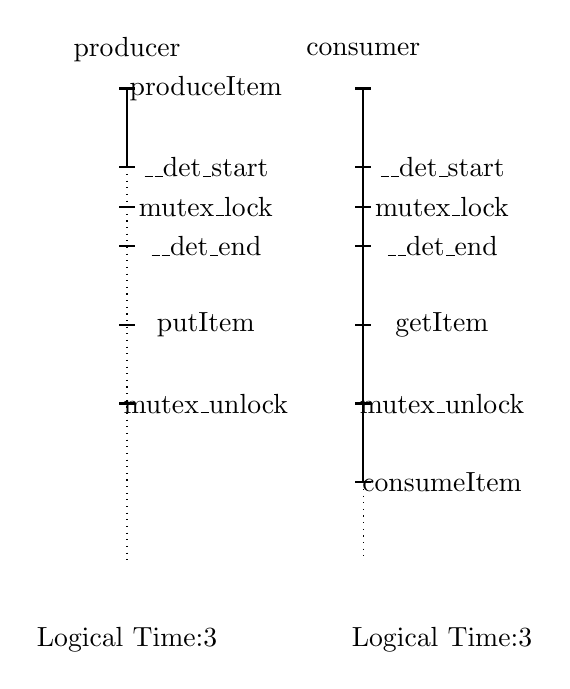
\begin{tikzpicture}
   \draw[thick] (0,4) --  (0,5); 
   \draw[dotted] (0,4) --  (0,-1);
   
   \node[align=right] at (0,5.5) {producer};
   \node[align=right] at (1,5) {produceItem};
   \draw[thick] (-0.1,5) -- (0.1,5);
   \node[align=right] at (1,4) {\_\_det\_start};
   \draw[thick] (-0.1,4) -- (0.1,4);
   \node[align=right] at (1,3.5) {mutex\_lock};
   \draw[thick] (-0.1,3.5) -- (0.1,3.5);
   \node[align=right] at (1,3) {\_\_det\_end};
   \draw[thick] (-0.1,3) -- (0.1,3);
   \node[align=right] at (1,2) {putItem};
   \draw[thick] (-0.1,2) -- (0.1,2);
   \node[align=right] at (1,1) {mutex\_unlock};
   \draw[thick] (-0.1,1) -- (0.1,1);   
   \node[align=right] at (0,-2) {Logical Time:3};
   
   \draw[thick] (3,0) --  (3,5); 
   \draw[dotted] (3,0) --  (3,-1);
   
   \node[align=right] at (3,5.5) {consumer};
   \node[align=right] at (4,5) {};
   \draw[thick] (2.9,5) -- (3.1,5);
   \node[align=right] at (4,4) {\_\_det\_start};
   \draw[thick] (2.9,4) -- (3.1,4);
   \node[align=right] at (4,3.5) {mutex\_lock};
   \draw[thick] (2.9,3.5) -- (3.1,3.5);
   \node[align=right] at (4,3) {\_\_det\_end};
   \draw[thick] (2.9,3) -- (3.1,3);
   \node[align=right] at (4,2) {getItem};
   \draw[thick] (2.9,2) -- (3.1,2);
   \node[align=right] at (4,1) {mutex\_unlock};
   \draw[thick] (2.9,1) -- (3.1,1);
   \node[align=right] at (4,0) {consumeItem};
   \draw[thick] (2.9,0) -- (3.1,0);
   \node[align=right] at (4,-2) {Logical Time:3};   
\end{tikzpicture}
\caption{An example of logical time imbalance. In this case the consumer has the token and already released the mutex, however consumeItem is taking too much time before it reaches \_\_det\_end again. At this time producer has to wait until consumeItem is finished and logical time of consumer becomes 4.}
\label{fig:p2-1}
\end{figure}

In Figure~\ref{fig:p2-1}, we show a particular execution point of the producer-consumer model that corresponds to the program shown in Figure~\ref{fig:p1-1}. In this case, consumer reaches consumeItem with logical time 3 and has the token. Assume the real execution time of consumeItem is 10s, which means that the next time the consumer reaches \_\_det\_end would be at least 10s later, before that consumer will hold the token. Which means the producer has to wait at \_\_det\_start for at least 10s. However we've already enforces the access order of the mutex, the execution out of the critical section should go in parallel since threads don't communicate at that part, this waiting time is totally unnecessary. In a more complex application with more synchronization, this kind of waiting will break a parallel program into a ser\subsection{Logical Time Imbalance}ial program.

From this case, we can make a conclusion: the logical time should precisely reflect the progress of the thread, only increasing the logical time by 1 at the end of synchronization is not enough. For this purpose, we add another system call just for adding logical time to the runtime. In Figure~\ref{fig:p2-2} we show that by increasing the logical time according to the execution time of consumeItem, the producer can proceed. Since this happens out of the deterministic area, as long as the logical time is increased in a deterministic manner, it won't break the determinism.

\begin{figure}
\centering
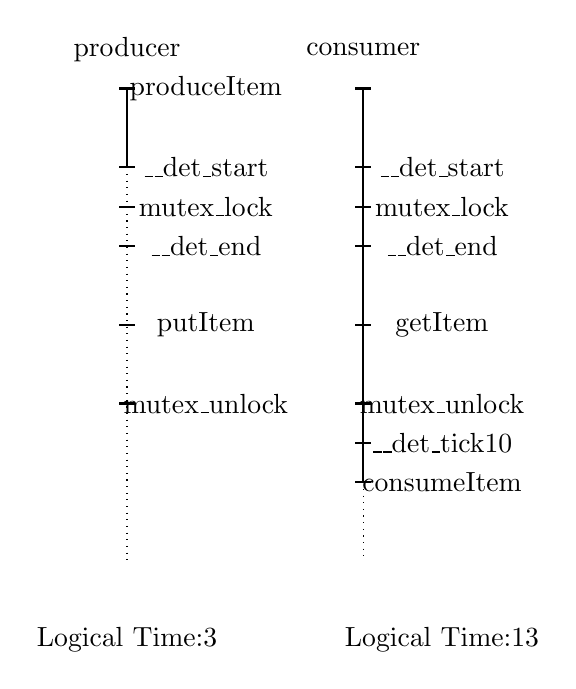
\begin{tikzpicture}
   \draw[thick] (0,4) --  (0,5); 
   \draw[dotted] (0,4) -- (0,-1);
   
   \node[align=right] at (0,5.5) {producer};
   \node[align=right] at (1,5) {produceItem};
   \draw[thick] (-0.1,5) -- (0.1,5);
   \node[align=right] at (1,4) {\_\_det\_start};
   \draw[thick] (-0.1,4) -- (0.1,4);
   \node[align=right] at (1,3.5) {mutex\_lock};
   \draw[thick] (-0.1,3.5) -- (0.1,3.5);
   \node[align=right] at (1,3) {\_\_det\_end};
   \draw[thick] (-0.1,3) -- (0.1,3);
   \node[align=right] at (1,2) {putItem};
   \draw[thick] (-0.1,2) -- (0.1,2);
   \node[align=right] at (1,1) {mutex\_unlock};
   \draw[thick] (-0.1,1) -- (0.1,1);   
   \node[align=right] at (0,-2) {Logical Time:3};
   
   \draw[thick] (3,0) --  (3,5); 
   \draw[dotted] (3,0) --  (3,-1);
   
   \node[align=right] at (3,5.5) {consumer};
   \node[align=right] at (4,5) {};
   \draw[thick] (2.9,5) -- (3.1,5);
   \node[align=right] at (4,4) {\_\_det\_start};
   \draw[thick] (2.9,4) -- (3.1,4);
   \node[align=right] at (4,3.5) {mutex\_lock};
   \draw[thick] (2.9,3.5) -- (3.1,3.5);
   \node[align=right] at (4,3) {\_\_det\_end};
   \draw[thick] (2.9,3) -- (3.1,3);
   \node[align=right] at (4,2) {getItem};
   \draw[thick] (2.9,2) -- (3.1,2);
   \node[align=right] at (4,1) {mutex\_unlock};
   \draw[thick] (2.9,1) -- (3.1,1);
   \node[align=right] at (4,0.5) {\_\_det\_tick\(10\)};
   \draw[thick] (2.9,0.5) -- (3.1,0.5);   
   \node[align=right] at (4,0) {consumeItem};
   \draw[thick] (2.9,0) -- (3.1,0);
   \node[align=right] at (4,-2) {Logical Time:13};   
\end{tikzpicture}
\caption{A solution for the logical time imbalance. Here we add the logical time of consumer by 10 before it reaches consumeItem, so that the producer can proceed without waiting for the consumer.}
\label{fig:p2-2}
\end{figure}

\section{Melchior}
In this section we present the detail design of Melchior. Melchior's runtime provides 2 system calls to define a deterministic area and 1 system call to bump the logical time. Melchior's compiler framework automatically instrument a program's so that every pthread synchronization is wrapped to be a deterministic area, and it can also find the best place and value to bump the logical time, achieving maximum scalability.

\subsection{Linux-Based Runtime Implementation}
The runtime is implemented purely in Linux kernel version 3.2.14. In order to not mess up some other running tasks in the OS, Melchior comes with a Linux namespace. Only the processes inside this namespace will affected by the deterministic scheduler. The namespace maintains a list of all the running tasks inside it, the list is ordered by PID.

Once the \_\_det\_start is called by a thread, the kernel will mark this thread as in a deterministic area, and check if the thread has the token, otherwise it removes the thread out of the current CPU run queue. When \_\_det\_end is called, the logical time will be increased by 1 and mark this thread as not in a deterministic area. Every time the logical time is updated, the runtime will put the token to the one that has the minimal logical time. If the thread that has the token is sleeping due to waiting on a token, the kernel will wake it up and put it back to the CPU run queue.

\subsection{LLVM-Based Compiler Framework}
\subsubsection{Pthread Annotation Pass}
This pass is very straightforward, it analysis the program's source code and puts \_\_det\_start and \_det\_end around the pthread sychronizations. With this pass all the pthread-based program can be made into deterministic-ready automatically. However a programmer can also manually put those two system calls into a program that has different threading model, even applicable for fork-based multi-process programs.

\subsubsection{Profile Pass}
As mentioned in Section ~\ref{imbalance}, we need to bump the logical time at certain places of the program, and it has to reflect the actual execution time of the program. In order to get the execution time of each section of a program, we make a profile pass to collect the execution time of each basic block, and then output the profile result to a file.

\subsubsection{Logical Time Pass}
After the program finished one profile run with the instrumentation of profile pass, the profiler will generate a file that encodes the execution time of each basic block. The logical time pass will take the profile data file as input, and compile the program again. This time at the end of each basic block, a \_\_det\_tick will be inserted with the parameter of the execution time of the current basic block.

\section{Evaluation}
The goal of our evaluation is to evaluate both the performance and correctness of our system. The evaluation was done on a server with 4 AMD Opteron 6376 processors, 64 cores in total, which is sufficient for the scalability evaluation.

\subsection{Correctness}
We evaluated Melchior with a variant of racey~\cite{hillstress}, which protects the shared memory access with mutexes. In our test, racey produces the same result for 2000 runs. And with some manually annotation work, two variants of racey that are implemented with fork instead of pthread, also passed the test for 2000 runs.

\subsection{Performance}
The workload we chose is pbzip2. It utilizes a typical producer-consumer model with selectable numbers of threads which is perfectly suitable for testing the scalability of our system.



\bibliographystyle{abbrv}
\bibliography{sigproc}  % sigproc.bib is the name of the Bibliography
\end{document}
